\begin{figure}[t]
  \UseAltLinespread
  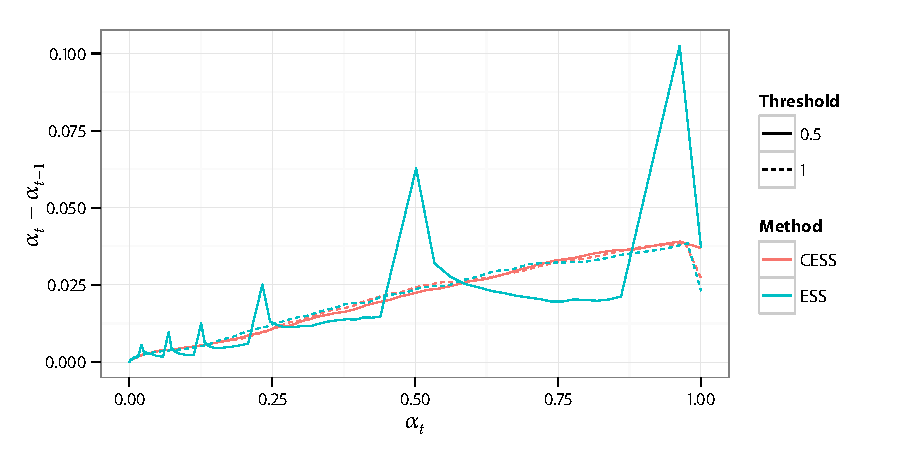
\includegraphics[width=\linewidth]{fig_src/Adaptive_Dist}
  \caption[Variations of the distribution specification parameter for the
  \protect\pet compartmental model using adaptive \protect\smc algorithms]
  {A typical plot of $\alpha_t - \alpha_{t-1}$ against $\alpha_t$ for the two-compartments \pet model with the simulated data set using the \smc[2] algorithm. The threshold is the value of $\ess/N$ below which resampling is performed. The specifications of the adaptive parameter (\ess or \cess) are adjusted such that all four samplers use roughly the same number of distributions (about 100).}
  \label{fig:adaptive_alpha}
\end{figure}
